\documentclass[]{article}
\usepackage{lmodern}
\usepackage{setspace}
\setstretch{1.5}
\usepackage{amssymb,amsmath}
\usepackage{ifxetex,ifluatex}
\usepackage{fixltx2e} % provides \textsubscript
\ifnum 0\ifxetex 1\fi\ifluatex 1\fi=0 % if pdftex
  \usepackage[T1]{fontenc}
  \usepackage[utf8]{inputenc}
\else % if luatex or xelatex
  \ifxetex
    \usepackage{mathspec}
  \else
    \usepackage{fontspec}
  \fi
  \defaultfontfeatures{Ligatures=TeX,Scale=MatchLowercase}
\fi
% use upquote if available, for straight quotes in verbatim environments
\IfFileExists{upquote.sty}{\usepackage{upquote}}{}
% use microtype if available
\IfFileExists{microtype.sty}{%
\usepackage{microtype}
\UseMicrotypeSet[protrusion]{basicmath} % disable protrusion for tt fonts
}{}
\usepackage[margin=2.0cm]{geometry}
\usepackage{hyperref}
\PassOptionsToPackage{usenames,dvipsnames}{color} % color is loaded by hyperref
\hypersetup{unicode=true,
            pdftitle={Application for Tenure-Track Instructor Position in Statistics at UBC},
            pdfauthor={Vincenzo Coia},
            colorlinks=true,
            linkcolor=Maroon,
            citecolor=Blue,
            urlcolor=Blue,
            breaklinks=true}
\urlstyle{same}  % don't use monospace font for urls
\usepackage{natbib}
\bibliographystyle{apalike}
\usepackage{longtable,booktabs}
\usepackage{graphicx,grffile}
\makeatletter
\def\maxwidth{\ifdim\Gin@nat@width>\linewidth\linewidth\else\Gin@nat@width\fi}
\def\maxheight{\ifdim\Gin@nat@height>\textheight\textheight\else\Gin@nat@height\fi}
\makeatother
% Scale images if necessary, so that they will not overflow the page
% margins by default, and it is still possible to overwrite the defaults
% using explicit options in \includegraphics[width, height, ...]{}
\setkeys{Gin}{width=\maxwidth,height=\maxheight,keepaspectratio}
\IfFileExists{parskip.sty}{%
\usepackage{parskip}
}{% else
\setlength{\parindent}{0pt}
\setlength{\parskip}{6pt plus 2pt minus 1pt}
}
\setlength{\emergencystretch}{3em}  % prevent overfull lines
\providecommand{\tightlist}{%
  \setlength{\itemsep}{0pt}\setlength{\parskip}{0pt}}
\setcounter{secnumdepth}{5}
% Redefines (sub)paragraphs to behave more like sections
\ifx\paragraph\undefined\else
\let\oldparagraph\paragraph
\renewcommand{\paragraph}[1]{\oldparagraph{#1}\mbox{}}
\fi
\ifx\subparagraph\undefined\else
\let\oldsubparagraph\subparagraph
\renewcommand{\subparagraph}[1]{\oldsubparagraph{#1}\mbox{}}
\fi

%%% Use protect on footnotes to avoid problems with footnotes in titles
\let\rmarkdownfootnote\footnote%
\def\footnote{\protect\rmarkdownfootnote}

%%% Change title format to be more compact
\usepackage{titling}

% Create subtitle command for use in maketitle
\providecommand{\subtitle}[1]{
  \posttitle{
    \begin{center}\large#1\end{center}
    }
}

\setlength{\droptitle}{-2em}

  \title{Application for Tenure-Track Instructor Position in Statistics at UBC}
    \pretitle{\vspace{\droptitle}\centering\huge}
  \posttitle{\par}
    \author{Vincenzo Coia}
    \preauthor{\centering\large\emph}
  \postauthor{\par}
      \predate{\centering\large\emph}
  \postdate{\par}
    \date{2019-12-13}


\begin{document}
\maketitle

{
\hypersetup{linkcolor=black}
\setcounter{tocdepth}{2}
\tableofcontents
}
\hypertarget{cover-letter}{%
\section{Cover Letter}\label{cover-letter}}

\textbf{NOTE: THIS APPLICATION IS A WORK-IN-PROGRESS}

Cover letter STATUS:

\begin{itemize}
\tightlist
\item[$\square$]
  Brain dump of ideas
\item[$\square$]
  Organization of ideas
\item[$\square$]
  Filling in gaps
\item[$\square$]
  Smooth over to form a draft
\item[$\square$]
  Complete: no changes needed.
\end{itemize}

Dear members of the search committee,

I am writing to enthusiastically apply for a tenure-track instructor position in Statistics (\href{https://www.stat.ubc.ca/three-tenure-track-instructor-positions-statistics-35876}{Job \#35876}). Ever since joining the department of Statistics full time in early 2017 to advance our Data Science initiatives, I've come to realize just how ideal of a fit the educational leadership stream is for me. My aim with this application is to indicate why this is so, as well as why the department and UBC (and external to UBC!) would benefit by promoting me to the educational leadership stream. An electronic version of my application can be found at \href{https://coia-ubc-application.netlify.com/}{coia-ubc-application.netlify.com}, and the content of this cover letter \href{}{here}.

Ultimately, in this position, I envision advancing all branches of Data Science education at UBC, especially through Statistics for Data Science. I'm equally excited to develop the new Minor in Data Science program as I am to continue developing the Master of Data Science (MDS) program. In fact, I'm actually rather torn between the two: there is still much to develop with MDS, and I'm rather invested in the program; but the allure of developing a new Minor program is a new equally exciting challenge that I can make valuable contributions to. Regardless of my level of involvement in these, I intend to keep an open stream of communication between the two programs, along with STAT 545A/547M, so that data science education at UBC can overall grow as a cohesive whole, as opposed to competing pieces.

My vision for doing this

I've identified four pillars of my career, which I hope will lay the foundation for my vision going forward in the teaching stream, as well as convey fit on my end. They are, in order of culmination:

\begin{enumerate}
\def\labelenumi{\arabic{enumi}.}
\tightlist
\item
  \textbf{Application}: addressing real problems with data science.
\item
  \textbf{Research}: discovering better ways to do data science.
\item
  \textbf{Development}: turning new research into programs and tools, which are ideally accessible to the public.
\item
  \textbf{Teaching}: spreading data literacy and enthusiasm to the public.
\end{enumerate}

Lastly, I'd like to elaborate on how my skills will be an asset to the department.

Excitement and promise for starting up the minor program, helping MDS and STAT 545A/547M evolve along with it.

hyperlinks to one or two examples of my teaching materials. Note that I don't see any of these as being ``finished'', but rather a work-in-progress.

\begin{itemize}
\tightlist
\item
  For STAT 545A/547M (Exploratory Data Analysis), I made the \href{https://stat545guidebook.netlify.com/}{lecture notes} and \href{https://stat545.stat.ubc.ca/}{course website}. Less relevant are Lectures 11+, taught by Dr.~Firas Moosvi, and Lecture 6, a guest lecture taught by my TA, Victor Yuan.
\item
  For DSCI 551 (Probability for Data Science), I wrote the \href{https://ubc-mds.github.io/DSCI_551_stat-prob-dsci/lectures/}{lecture notes} by using Dr.~Mike Gelbart's notes from the previous year as scaffolding.
\item
  I'm writing an open-source book on regression analysis for data science, called \href{https://interpreting-regression.netlify.com/}{Interpreting Regression}. It's in its early stages.
\end{itemize}

What I'm comfortable teaching (useful in parallel to the minor program in DS)

Tools; my comfort level with CS. Although I don't have formal training in CS outside of perhaps a few undergraduate courses, my approach to learning these things is to identify tools and techniques that would be useful, and commit to building these tools. I prefer this approach over prescribed training such as online courses, because I find it more genuine as I encounter concepts as they become relevant. For example, I've been learning web hosting as I've been learning about Hugo, blogdown, and netlify to create websites like my homepage, course websites like STAT 545A/547M, and hosting ``books'' such as Interpreting Regression online. I've learned shell scripting back in my PhD, and continue to learn more, as I embrace GNU Make and workflow automation in general.

Teaching tools and methods

In this application, I'll show you how my career goals are related to teaching and educational leadership. You'll read about my plans to continue reframing statistics for the purpose of data science by writing books such as interpreting regression and writing software such as dist fire.

the names of three references who have been asked to send reference letters:

\begin{enumerate}
\def\labelenumi{\arabic{enumi}.}
\tightlist
\item
  Dr.~Tiffany Timbers (current supervisor)
\item
  Dr.~Michael Gelbart (current supervisor)
\item
  Dr.~Harry Joe (PhD supervisor)
\end{enumerate}

I am eager to begin the position on the indicated July 1, 2020 start date, but am ultimately flexible.

Enthusiastically yours,

Vincenzo Coia, PhD

\url{https://vincenzocoia.com/}

\hypertarget{curriculum-vitae}{%
\section{Curriculum Vitae}\label{curriculum-vitae}}

\hypertarget{work-experience}{%
\subsection{Work Experience}\label{work-experience}}

2017/01 - present\\
\textbf{Lecturer of Data Science}\\
(Initially: Postdoctoral Teaching and Learning Fellow)\\
Masters of Data Science Program, and the Department of Statistics\\
The University of British Columbia\\
Vancouver, BC

2009/05 - 2014/05\\
\textbf{Short-term statistical consulting} (6 projects)\\
UBC and private

\hypertarget{education}{%
\subsection{Education}\label{education}}

\textbf{PhD in Statistics}\\
2012/09 - 2017/02\\
The University of British Columbia\\
Conferred May 29, 2017

\textbf{MSc in Mathematics and Statistics (Statistics)}\\
2011/09 - 2012/08\\
Brock University\\
Conferred on October 13, 2012

\textbf{BSc (3-year) in Biological Sciences}\\
Minor in Earth Sciences\\
2005/09 - 2011/04\\
Brock University\\
Conferred ``With Distinction'' on October 22, 2011

\textbf{BSc (Honours) Mathematics Integrated with Computers and Applications}\\
Concentration in Statistics\\
2005/09 - 2011/04\\
Brock University\\
Conferred ``With First-Class Standing'' on June 7, 2011

\hypertarget{volunteer-positions}{%
\subsubsection{Volunteer Positions}\label{volunteer-positions}}

2016/09 - 2016/02\\
\textbf{Science World at TELUS World of Science }\\
Vancouver, BC\\
78.15 hours

2013/10 - 2014/05\\
\textbf{Beaty Biodiversity Museum: Events Volunteer}\\
Vancouver, BC\\
35.0 hours

2013/04 - 2013/09\\
\textbf{UBC Farm}\\
Vancouver, BC\\
102.5 hours

2011/06 - 2011/08\\
\textbf{Project S.H.A.R.E. community garden}\\
Niagara Falls, ON\\
15.0 hours

\hypertarget{research-assistantships}{%
\subsubsection{Research Assistantships}\label{research-assistantships}}

2013/05 - 2013/08\\
\textbf{Robust penalized regression}\\
Supervisor: Dr.~Gabriela Cohen-Freue\\
Department of Statistics\\
The University of British Columbia\\
Vancouver, BC

2012/05 - 2012/08\\
2011/05 - 2011/08\\
2010/05 - 2010/08\\
\textbf{Extreme value modelling}\\
Supervisor: Dr.~Mei Ling Huang\\
Department of Mathematics\\
Brock University\\
St.~Catharines, ON

2010/09 - 2011/06\\
\textbf{Quantum monte carlo simulations}\\
Supervisors: Dr.~Stuart Rothstein; Dr.~Wai Kong (John) Yuen\\
Department of Chemistry and Department of Mathematics\\
Brock University\\
St.~Catharines, ON

\hypertarget{teaching-assistantships}{%
\subsubsection{Teaching Assistantships}\label{teaching-assistantships}}

\textbf{Duration}: From the latter part of my undergrad, to the end of my PhD.

UBC:

\begin{itemize}
\tightlist
\item
  \textbf{SCIE 300: Communicating Science} (5x)
\end{itemize}

Brock University:

\begin{itemize}
\tightlist
\item
  \textbf{MATH 4P82/5P82: Non-parametric Statistics}
\item
  \textbf{MATH 3P82: Regression Analysis}
\item
  \textbf{MATH 4P81/5P81: Sampling Theory}
\item
  \textbf{MATH 3P81: Experimental Design} (2x)
\item
  \textbf{MATH 2F40: Mathematics Integrated w/ Computers and Applications II}
\end{itemize}

\hypertarget{publications-and-talks}{%
\subsection{Publications and Talks}\label{publications-and-talks}}

\hypertarget{articles-submitted-to-refereed-journals}{%
\subsubsection{Articles Submitted to Refereed Journals}\label{articles-submitted-to-refereed-journals}}

\begin{itemize}
\item
  Huang, M.L., Coia, V., and Brill, P.H. (2013) A cluster truncated
  Pareto distribution and its applications. ISRN Probability and
  Statistics 2013: Article ID 265373.
\item
  Ayad, M., Coia, V., and Kihel, O. (2014) The number of relatively
  prime subsets of a finite union of sets of consecutive integers.
  Journal of Integer Sequences 17: Article 14.3.7
\item
  Coia, V., and Huang, M.L. (2014) A sieve model for extreme
  values. Journal of Statistical Computation and Simulation.
  84(8):16921710.
\end{itemize}

\hypertarget{articles-submitted-to-conference-proceedings}{%
\subsubsection{Articles Submitted to Conference Proceedings}\label{articles-submitted-to-conference-proceedings}}

\begin{itemize}
\tightlist
\item
  Huang, M. L., Coia, V., and Brill, P.H., A mixture truncated
  Pareto distribution, In JSM Proceedings 2012, Statistical Computing
  Section, Alexandria, VA: American Statistical Association, pp.

  \begin{enumerate}
  \def\labelenumi{\arabic{enumi}.}
  \setcounter{enumi}{24882497}
  \item
  \end{enumerate}
\end{itemize}

\hypertarget{conference-and-roundtable-contributions}{%
\subsubsection{Conference and Roundtable Contributions}\label{conference-and-roundtable-contributions}}

\begin{itemize}
\item
  Coia, V., Nolde, N., and Joe, H. Forecasting Extremes for Flooding
  (Invited Talk). The 44th Annual Meeting of the Statistical Society
  of Canada. May 29June 1, 2016 at Brock University, St.~Catharines,
  ON.
\item
  Coia, V., and Jeanniard du Dot, T. (Invited Demonstration) ``Using
  the Grammar of Graphics and Interactivity to explore Biologging Data
  in R''. May 6, 2015. Building a Bioanalytical Theory for Analysis of
  Marine Mammal Movements: A Peter Wall International Research
  Roundtable. The University of British Columbia, Vancouver, BC.
\item
  Coia, V. ``Flood Warning: An Application of High-Quantile Regression''
  (Contributed Talk). SFU/UBC Joint Graduate Student Seminar (Winter).
  February 28, 2015 at the SFU Harbour Centre, Vancouver, BC.
\item
  Coia, V. ``A New Sieve Model for Extreme Values'' (Contributed Talk).
  SFU/UBC Joint Graduate Student Seminar (Fall). September 29, 2012 at
  the SFU Harbour Centre, Vancouver, BC.
\item
  Coia, V., and Huang, M.L. ``On Estimation of Heavy Tailed
  Distributions'' (Contributed Talk). The 40th Annual Meeting of the
  Statistical Society of Canada. June 36, 2012 at the University of
  Guelph, Guelph, ON.
\item
  Huang, M.L., Coia, V., and Brill, P.H. ``A Mixture Truncated Pareto
  Distribution'' (Contributed Talk). The 2012 Joint Statistical
  Meetings. July 28August 2, 2012 at San Diego, California
\end{itemize}

\hypertarget{awards}{%
\subsection{Awards}\label{awards}}

\hypertarget{university-issued}{%
\subsubsection{University Issued}\label{university-issued}}

\begin{itemize}
\tightlist
\item
  2012/09 - 2016/08: Four-Year Fellowship
\item
  2012/09 - 2016/08: Faculty of Science Graduate Award
\item
  2011/09: Dean of Graduate Studies Excellence Scholarship
\item
  2011/06/07: Dean's Gold Medal
\item
  2011/06/07: Distinguished Undergraduate Student Award in Mathematics
\item
  2011/03: President's Surgite Award
\end{itemize}

\hypertarget{nationally-recognized}{%
\subsubsection{Nationally Recognized}\label{nationally-recognized}}

\begin{itemize}
\tightlist
\item
  2013/06: Governor General of Canada's Gold Medal
\item
  2012/09 - 2015/08: NSERC Postgraduate Award (Doctoral, 3-year)
\item
  2011/09 - 2012/08: NSERC Alexander Graham Bell Canada Graduate Scholarship (Masters)
\item
  2010/05 - 2010/08: NSERC Undergraduate Student Research Award
\end{itemize}

\hypertarget{individual-donors}{%
\subsubsection{Individual Donors}\label{individual-donors}}

\begin{itemize}
\tightlist
\item
  2012/04: Dr.~Jack Lightstone \& Dorothy Markiewicz Scholarship
\item
  2012/04: Dr.~Raymond \& Mrs.~Sachi Moriyama Grad. Fellowship
\item
  2012/03: Tomlinson Entrance Scholarship for Excellence in Mathematics and Science
\item
  2011/06: John and Roslyn Reed Book Prize
\item
  2010/09: Art Bicknell Scholarship in Mathematics
\item
  2010/09: Ian D. Beddis Family Scholarship
\item
  2010/09: Terry and Sue White Mathematics and Science Scholarship
\item
  2007/09: M.J. (``Mel'') Farquharson Scholarship
\item
  2006/09: Scholler Foundation Scholarship in Chemistry
\end{itemize}

\hypertarget{athletic-awards}{%
\subsubsection{Athletic Awards}\label{athletic-awards}}

\begin{itemize}
\tightlist
\item
  2016/04/03: Sportsmanship Award, UBC Thunderbirds Sport Clubs (Fencing)
\item
  2016/02/28: Bronze Medal in Senior Mixed Epee (Intercollegiate Tournament, UBC)
\item
  2015/11/16: Bronze Medal in Senior Mixed Epee (Remembrance Day Tournament, UBC)
\item
  2012/03/28: RM Davis Surgite Award
\item
  2009/12/12: First Place Award Winter Epeedemic, Toronto Fencing Club
\item
  2009/03: Varsity Fencing Rookie of the Year Award
\end{itemize}

\hypertarget{declined-awards}{%
\subsubsection{Declined Awards}\label{declined-awards}}

\begin{itemize}
\tightlist
\item
  2012/04: Ontario Graduate Scholarship (Doctoral)
\item
  2011/05: Ontario Graduate Scholarship (Masters)
\end{itemize}

\hypertarget{professional-activities}{%
\subsection{Professional Activities}\label{professional-activities}}

Dept. of Statistics, The University of British Columbia:

\begin{itemize}
\tightlist
\item
  2016/05 - 2016/06: \textbf{Search committee member (for CRC 2 faculty position)}
\item
  2015/04/30: \textbf{Organizer of the ``\href{http://stat.ubc.ca/~vincen.coia/abstractworkshop.html}{How to Write an Awesome Abstract}'' workshop}
\item
  2014/06 - 2015/05: \textbf{Organizer of the \href{http://stat.ubc.ca/~vincen.coia/seminar.html}{SFU/UBC Joint Seminar}}
\item
  2014/06 - 2014/09: \textbf{Organizer of the Graduate Student Trip}
\item
  2014/04 - 2015/05: \textbf{Co-founder of the Graduate Writing Forums}
\item
  2013/06 - 2014/05: \textbf{Statistics Graduate Student Representative}
\end{itemize}

\hypertarget{statement-of-vision-for-education-in-statistics-and-data-science}{%
\section{Statement of vision for education in statistics and data science}\label{statement-of-vision-for-education-in-statistics-and-data-science}}

STATUS:

\begin{itemize}
\tightlist
\item[$\boxtimes$]
  Brain dump of ideas
\item[$\boxtimes$]
  Organization of ideas
\item[$\boxtimes$]
  Filling in gaps
\item[$\boxtimes$]
  Smooth over to form a draft
\item[$\square$]
  Complete: no changes needed.
\end{itemize}

A major passion of mine is reframing Statistical Science from the lens of Data Science, by taking a ``problem-first'' approach. You can read about my vision in the first section, which is followed by a section describing how I go about executing this vision as educational leadership initiatives.

\hypertarget{statistics-for-data-science}{%
\subsection{Statistics for Data Science}\label{statistics-for-data-science}}

Why does Statistics need reframing for Data Science? Statistical Science tends to begin with assumptions / a modelling framework, then describing properties and methods that enable solutions to a problem. This is a ``framework-first'' approach. But Statistics for Data Science requires a ``problem-first'' approach, focussing on how to appropriately construct a modelling framework from real-world problems. These two approaches are not translatable, because real problems don't neatly satisfy assumptions nor come with a description of what output is appropriate for addressing the problem. A real problem requires critical evaluation as to what outputs and what assumptions are useful and realistic. This isn't assumption-\emph{checking}, it's assumption-\emph{building}.

By the way, even Applied Statistics might sometimes seem to take a problem-first approach, because it starts with a motivating problem. But the focus is still on describing properties of the newly defined framework, falling squarely within the field of Statistical Science. On the other hand, Statistics for Data Science must focus on how to deal with a wide range of problems, not just one problem type. This is a challenge that relies on the properties already described by Statistical Science, hence why both approaches are important!

My viewpoint on this has largely come about through the re-development of many courses and materials throughout the years. Formal redevelopments (or developments) included DSCI 531/532, DSCI 561/562, and BAIT 509; just about all other courses I've been involved with have had some level of redevelopment, such as STAT 545A/547M, DSCI 511, DSCI 574, and DSCI 551, amongst others.

The way I see it, teaching a problem-first approach for Statistics for Data Science still has a long way to go. A central and powerful approach that I've been adopting is to create content focussing on the \emph{type of problem} encountered in real-world problems, instead of the traditional Statistics topics. Perhaps the best example of this is DSCI 562 (Regression II), which I re-developed last year. Instead of teaching ``Survival Analysis'' and ``Multiple Imputation'', I teach ``regression when data are censored'' and ``regression when data are missing''. This changes the focus of the lessons to be about evaluating approaches for solving the type of problem, including evaluating the impact of ignoring the problem altogether (perhaps there's little to no impact!). This approach allows students to creatively come up with solutions to a variety of real world problems, which are sure to involve ``combined'' scenarios, such as a censored response with some missing data.

Sometimes, a traditional statistical topic is made up of more than one type of problem, resulting in a restricted way of thinking. For example, the topic of Generalized Linear Models (GLM's) can be split into two problems: regression when the range of the response is restricted, and using a distributional assumption to improve estimation performance. Both are valuable tools that expand beyond the scope of GLM's, but if just taught as GLM's, restricts students' thinking to the smaller range of problems that GLM's can handle.
Determining the type of problem that a traditional statistical topic addresses is not always obvious. I found the GLM example to be tricky; here are some other tricky ones, from DSCI 551 (Probability for Data Science):

\begin{itemize}
\tightlist
\item
  ``Probability Distributions'' has the underlying problem of communicating an uncertain outcome.
\item
  ``Simulation'' has the underlying problem of calculating probabilistic quantities (mean, probabilities, etc.) when the distributions or calculations are hard to come by.
\item
  ``Independence'' is tricky because it's really ``dependence'' that is more interesting. Dependence, then, can have an underlying problem of garnering information from a dependent variable (or what I like to call ``harvesting dependence'').
\end{itemize}

This problem-first approach naturally promotes motivation in the classroom, because the topics are designed to be practical from the get-go. Sample real-world problems become important, and where possible, I draw from my capstone and industry experience to create compelling examples. Perhaps my favourite is the \href{https://ubc-mds.github.io/DSCI_551_stat-prob-dsci/lectures/simulation.html\#multi-step-simulations-10-min}{``ships making demands at the port'' example in DSCI 551}, which I encountered in one of last year's capstone projects, to demonstrate simulation under a more complicated situation. Another favourite is flood forecasting; another, determining the effect of blue-light-blocking glasses on sleep.

An interesting thing that happens when taking a problem-first approach is that it brings to light areas of Statistics that are useful, yet are not receiving much attention. Two examples are quantile regression or distributional forecasting instead of mean regression. Another example is extreme value modelling (EVM), which becomes invaluable for problems that have heavy tailed data, such as at least one capstone project from Seahorse Strategies last year (the team should have used EVM, but did not, because we didn't teach it in MDS), as well as organizations tackling the issue of flood forecasting and flood frequency assessments. Interestingly, these topics tend to be deemed difficult, probably because of our community's obsession with the mean, as well as a general misunderstanding of the role of distributions outside of just being a ``necessary statistical assumption''. I believe these topics are more accessible than they're made out to be, if taught from a problem-first lens, because the mathematical details are inconsequential.

\hypertarget{educational-leadership}{%
\subsection{Educational Leadership}\label{educational-leadership}}

I'm finding that there's a general lack of problem-first education in Statistics, as well as a lack of good examples, but this presents opportunity. I envision being a leader in building Statistics for Data Science -- it's actually a major component of my career and my life. This section describes my strategy plan for having an impact both within and outside of the classroom walls, including some of the things that I've accomplished already.

Perhaps the simplest approach I've taken is making my course material public, which I intend to continue doing. People are starting to notice. See the figure for activity from my most recent tweet of my most recent release, for DSCI 551. Also, the \href{https://stat545guidebook.netlify.com/}{STAT 545A/547M content} is still receiving a lot of global attention, largely thanks to Dr.~Jenny Bryan's original efforts with the course (although the content needs more upgrading than I've had capacity to supply).

\begin{figure}
\centering
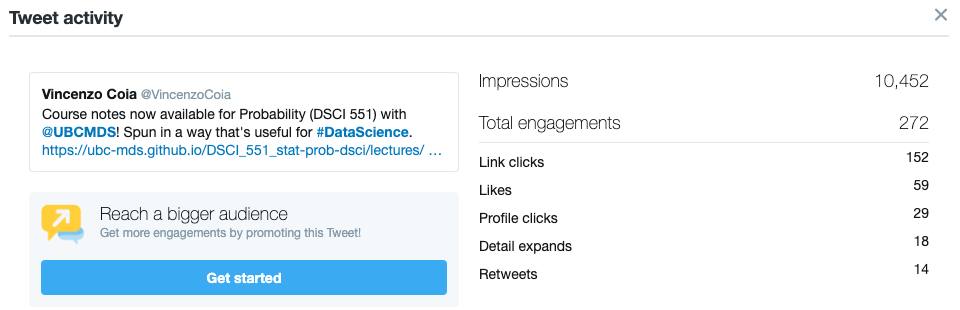
\includegraphics{./img/551_tweet.png}
\caption{DSCI 551 tweet activity}
\end{figure}

I like to think beyond the structure of a classroom, by developing material intended to be used by a wider range of people than those who refer to course notes. So far, this means writing a book focussing on regression analysis from a problem-first perspective. It's far from done, but it's also far from just starting out. I'm calling it ``\href{https://interpreting-regression.netlify.com/}{Interpreting Regression}''. For maximum return on investment, I try to write course notes that can be easily adapted to the wider audience of the book. I believe distributional forecasting deserves its own book as well, and would include approaches like extreme value modelling, and techniques like copula modelling. These topics are more practical and accessible than people think.

I also see the need for new R packages for making Statistics more accessible for Data Science. I made some S3 Object Oriented R packages during my PhD with many useful functions, but being my first R packages, they have many deficiencies, including a lack of vignettes, too many overly complicated functions, and a lack of tests. I have ideas for packages to replace these older ones, as well as altogether new ones. My goal for each one is to submit each to CRAN and ROpenSci, publishing a corresponding paper to the Journal of Statistical Software, as well as making helpful vignettes. Here are my ideas:

\begin{itemize}
\tightlist
\item
  The \href{https://github.com/vincenzocoia/distplyr/}{\texttt{distplyr}} package (which is already underway) will make it easier to work with univariate distributions, including empirical ones, for the promotion of distribution-based analyses. This makes a distribution an S3 object, which can then be manipulated. This would, for example, aid in the teaching of mixture distributions, and aid in the creation of extreme value models using functions like \texttt{distplyr::right\_graft()} or \texttt{distplyr::left\_graft()}.
\item
  The \href{https://github.com/vincenzocoia/coperate/}{\texttt{coperate}} package is similar to \texttt{distplyr} in that it makes it easier to work with copulas by making a copula an S3 object. This will replace the \href{https://github.com/vincenzocoia/copsupp/}{\texttt{copsupp}} package, one of my deficient R packages from my PhD days, yet still has lots of useful functionality.
\item
  Modelling packages to go alongside the above two.
\end{itemize}

In short, I'm aiming to lead the development of a suite of tools that have a ``wow'' quality, so that they become go-to resources for people needing help for Statistics for Data Science to satisfy their unique needs. Aside from books, public course content, and R packages that I've mentioned above, I'm curious as to what other medium would appeal to other aspects of learning. R shiny web apps is one such medium that is on my radar. For example, the impact of multicollinearity is much easier to grasp by visualizing a regression plane slicing a data cloud, allowing the user to change the correlation between the covariates. Other media are only in the space of my imagination, but that's where things begin! Maybe one day I will in fact start an engaging podcast with my colleagues, or curate a monthly ``Statistics for Data Science Box'' containing books or other resources for busy professionals wanting to grow and learn. The possibilities are endless.

A completely different area where I would like to provide leadership is in teaching educators how to go about teaching Statistics for Data Science, because the field is so new. I of course don't have all the answers, so perhaps the best medium for this is to host a workshop / conference on Data Science education. In fact, I've already helped kick off a vision for such a workshop by spearheading the creation of a vision for MDS. Related, I believe it's important to be stewards of Data Science by promoting responsible use, which is reflected in our material, but also in this workshop / conference.

Because a problem-first approach is so critical for Statistics for Data Science, I believe a final area of leadership is to exercise my data science skills, or as Stephen Covey says in his book ``The 7 Habits of Highly Effective People'', to ``sharpen the saw''. Just as it's important for us to take time to stay healthy, it's also important as an educator to keep my Data Science skills sharpened, as well as up to pace with a changing field. Whether or not this is considered EL, it's important so that I can give students the most relevant and best education I can possibly give. Simple ways of remaining sharp, or at least up to date, is to subscribe to relevant newsletters such as RStudio's and ROpenSci's, and stay involves with the Data Science community on Twitter. But I believe it's important to actually do a bit of work for external organizations to help them with their data science needs. I did this last summer with BGC Engineering by dedicating a small amount of time each week, and this opened my eyes to their values and their data science problems, which I can then bring back to the classroom.

\hypertarget{statement-of-teaching-and-training-philosophy}{%
\section{Statement of teaching and training philosophy}\label{statement-of-teaching-and-training-philosophy}}

\hypertarget{teaching-philosophy}{%
\subsection{Teaching Philosophy}\label{teaching-philosophy}}

STATUS:

\begin{itemize}
\tightlist
\item[$\boxtimes$]
  Brain dump of ideas
\item[$\boxtimes$]
  Organization of ideas
\item[$\boxtimes$]
  Filling in gaps
\item[$\boxtimes$]
  Smooth over to form a draft
\item[$\square$]
  Complete: no changes needed.
\end{itemize}

My philosophy on teaching can best be broken down into four categories: \textbf{appropriate course structure}, \textbf{responsive teaching}, \textbf{motivation}, and \textbf{self-improvement}.

\hypertarget{appropriate-structure}{%
\subsubsection{Appropriate Structure}\label{appropriate-structure}}

You and I don't really know English. We only know enough for it to be a sufficiently useful tool for our own daily activities. I take this concept to heart as I design and deliver my courses. It's fallacious to design a course around \emph{topics}, but rather on building \emph{skills} for a certain purpose. To me, these skills formulated as a list of \textbf{learning objectives} (LO's) act as a ``true north'' that all components of a course point towards, and are the most important structure to the course. For example, course content on the topic ``heteroskedasticity'' could be developed in many directions. The students, thinking they have to ``know heteroskedasticity'', get stuck studying its never-ending scope. Instead, a learning objective such as ``modify a linear model to appropriately incorporate heteroskedasticity based on data diagnostics'' provides direction for the teaching team to create material, and clarity for the students. For concrete examples, take a look at \href{https://ubc-mds.github.io/DSCI_551_stat-prob-dsci/lectures/}{the DSCI 551 notes}, or my other course materials.

Clarity about the course structure and expectations is important for equipping students with a map of what they need to do to succeed. In addition to discussing how students should use the LO's, describing the summative assessments and a course syllabus is also important, as well as making it easy to navigate course material (see, for example, the \href{https://stat545.stat.ubc.ca/}{STAT 545A/547M syllabus website}). Informing the students of any changes or of any mistakes, no matter how painful, is also critical for maintaining clarity.

\hypertarget{responsive-teaching}{%
\subsubsection{Responsive teaching}\label{responsive-teaching}}

Too much structure can stymie a course. This is because, while preparing course material, the instructor is not truly equipped with the clarity of how to most appropriately deliver material until the material has been delivered. For example, a question for the class might have seemed insightful when it was being prepared, but maybe during class the question doesn't end up being insightful. Or, maybe the lecture delivery time was underestimated. The answer to addressing this issue is responsive teaching.

Responsive teaching to me is about staying in touch with the class to get a feel for areas that need more or less attention. For example, it means: taking a break when the energy of the class is low; responding to class confusion by explaining something in a different way on the whiteboard; or spending more or less time on something after realizing its importance mid-class. In this way, teaching is more akin to improv comedy, where actors must respond to random cues from the audience (I've taken lessons). I believe in embracing a mindset of letting go and trusting in yourself to respond appropriately the moment things go off course, and to also be humble and admit when you don't know something. This type of spontaneity sometimes also requires realizing and appropriately acting on your agency in adapting a course on the fly. Understanding that a course is flexible allows you to be nimble during contact hours with students, as opposed to feeling stuck in delivering the course exactly as it was originally laid out. However, it's important to be strategic when making changes so that things remain orderly and as seemless as possible for the students, and to be clear about any changes made. I like using the start of class to check in and return to a roadmap of the course so that everyone remains on board a moving bus.

Contact time with students is critical for adapting my teaching to the students, and provides tremendous value for students to actually enrol in a program as opposed to taking an online course. Perhaps the most effective method for doing this is making a point to engage with each student in lab. Equally as powerful are discussion-style office hours. I no longer hold my office hours in my office, because the office hour model whereby students just drop by to ask a question is just not effective. There ends up being a queue of students, usually asking common questions, and these students feel pressured to leave the office so that others can get a turn. Instead, I hold my office hours in a lab-like room suitable for collaboration. I end up leading a whole-group discussion prompted by student questions. This gives me even more insight as to how things are going in class, and allows me the opportunity to modify the course moving forward or make clarifications.

Some other methods for connecting with the students are:

\begin{itemize}
\tightlist
\item
  being present on the course Slack channel (and sometimes even other course channels) to provide more insight,
\item
  sending out a 1-minute long early survey about how the course is going,
\item
  taking the time to talk to students who approach me during the mid-class break or after class,
\item
  pausing to ask questions and check for insight in the classroom,
\item
  applying active learning strategies such as think-pair-share or live coding, and
\item
  checking in to see how things are going at the start of each class, by asking questions like ``how are we feeling about the quiz coming up next week'', or ``how are we feeling this week''.
\end{itemize}

\hypertarget{motivation}{%
\subsubsection{Motivation}\label{motivation}}

Neither structure nor responsive teaching will suffice if the students don't know the reason for discussing the course material.

I take to heart what I learned from Greg Wilson, that teaching is much more about motivating students than it is knowledge transfer. Students have access to any information they want through the internet, but a classroom environment has the powerful advantage of the presence of peers and an engaging instructor. On the teaching front, this means being enthusiastic, and focussing on why they should care about the things I talk about. It also means being aware of the lengthy (usually 80-minute) time frame that students are present for (and that's just for one class), by taking a break mid-class, returning to the big-picture, and providing additional instructions for exercises for people who may have ``fallen off the bus''. I'm pleased that I regularly receive ample praise on my instructor evaluations, and I encourage you to take a look.

\hypertarget{self-improvement}{%
\subsubsection{Self-Improvement}\label{self-improvement}}

What's better than effective teaching? Teaching that continually becomes more effective.

Community engagement is one method to become a better teacher. This means keeping an open dialogue and sharing experiences with other teachers, especially my colleagues. Aside from simple acts like sharing ideas and experiences through Slack and gatherings, I'm proud that my team gives and receives formative feedback on our teaching by visiting each others' lectures.

An after-action review is another effective method, involving capturing the insight you gain after teaching. There are three ways I engage in an after-action review. First, I capture regular insight throughout the delivery of the course as GitHub Issues, so that the insight can easily be referred to in the future and by any of my colleagues. Secondly, I find keeping a teaching journal that's not tied to a specific course is useful for becoming a better teacher in general -- and it's even easier now that my team has our lectures recorded. Thirdly, my colleagues and I engage in a ``retreat'' at the end of each term, to discuss our insight on our courses and the MDS program as a whole.

Realizing one's own struggles is also critical for self-improvement. For now, one thing I struggle with are student names. I feel embarrassed to use names because I'm sure to make mistakes, but calling students by their name is important because it shows that the instructor cares. I already review class lists, but have been stepping outside of my comfort zone by no longer avoiding using names. Another thing I struggle with is writing in an orderly fashion on the whiteboard. I use the whiteboard for spontaneity / responsive teaching, which means I don't know how I'll ultimately be using the board throughout the class. I end up running out of space, and end up using the board in a non-linear fashion, which can sometimes be confusing. For now, I intend to remain mindful of this and keep practicing.

\hypertarget{training-philosophy}{%
\subsection{Training Philosophy}\label{training-philosophy}}

STATUS:

\begin{itemize}
\tightlist
\item[$\boxtimes$]
  Brain dump of ideas
\item[$\boxtimes$]
  Organization of ideas
\item[$\boxtimes$]
  Filling in gaps
\item[$\boxtimes$]
  Smooth over to form a draft
\item[$\square$]
  Complete: no changes needed.
\end{itemize}

When it comes to training, I aim to foster a clear and highly communicative environment between me and my trainees.

Examples of group leadership include the development and delivery of courses with colleagues and teaching assistants, and the delivery of capstone projects together with partner organizations and student groups with MDS. I believe effective group leadership involves establishing everyone's roles, expectations, and time commitments; creating an empowering work culture for all group members; and defining success. When training is involved, delegation and feedback are key to promote the subordinate's growth.

Clarifying each team member's role, expectations, and level of authority for making decisions is the beginning step in defining a framework for which the group can operate effectively. Doing so allows everyone to respect each other's time and boundaries, so that group members know how to interact with each other. The MDS Capstone projects are one example, where I feel it is tremendously important to immediately clarify the roles of the student group, the partner organization, and myself, so that problems don't arise such as the partner organization treating the students like employees. Another example is having established roles at the beginning our DSCI 561 redevelopment kickoff meeting, involving a graduate assistant to be the main one putting ``pen to paper'', myself as her mentor, and colleagues for checking in with the high-level direction of the redevelopment.

When it comes to the actual nature of the interactions between group members and myself, I believe it's important to empower all group members to feel some ownership over the project that they can make a valuable contribution to. The reality is that everyone has a unique set of skills that, when tapped, result in a better end product than I could have produced on my own. Doing this means to be deliberate about my interactions -- it means bringing positive and friendly energy, being aware of my facial expression, and considering all input and ideas as if they are thoughtful. Setting up the environment like this also helps create a culture that's safe for dissent, which also involves asking everyone to feel comfortable to disagree with others. It's also important to show every member respect, for example, by treating them as if their time is valuable, such as by allowing them to meet either electronically or in person (if appropriate). Finally, it's important to show gratitude and to sometimes just stop and marvel at what has been created.

When it comes to the actual teaching and training of my trainees, it's important to provide regular input both verbally and as written feedback. This involves taking the time to write detailed notes as to where they can improve or where they are exceeding expectations. For example, my capstone groups know that I will give them the courtesy of looking into the details of their work and give them detailed feedback. This is more time consuming than just skimming over their work and providing a few comments, but this is what promotes learning.

Another important aspect of training is to delegate, especially when it comes to those tasks that we as leaders feel more skilled at. This is difficult, because we feel ownership over our tasks. We feel that we are in the best position to do the job, and we gain the satisfaction when they are done. But we must let go, and ``gift'' these tasks to our trainees who are less skilled at it, because the challenge it presents them is a powerful learning opportunity. Of course, this doesn't mean gifting and walking away. As mentioned, regular feedback is important. For example, I like to give my teaching assistants the opportunity to teach up to one lecture for most courses that I teach. I provide guidance leading up to the lecture, and afterwards, I like to walk with them outdoors and allow them to tell me how they think the lecture went. I find that simply lending an ear and asking questions provides the space for reflection and learning, and I hear how valuable this experience is for them.

Finally, as in teaching, I always looking for ways to improve my leadership in training. This involves asking the uncomfortable question of how I'm doing as a leader. For me, as I learned from last year's capstone project, I need to be more mindful of group dynamics. Even if things between me and each team member or student is fine, the relationship between other team members might not be. This year, I'll be meeting with each student individually early on to see how things are going.

\hypertarget{diversity-statement}{%
\section{Diversity Statement}\label{diversity-statement}}

STATUS:

\begin{itemize}
\tightlist
\item[$\square$]
  Brain dump of ideas
\item[$\square$]
  Organization of ideas
\item[$\square$]
  Filling in gaps
\item[$\square$]
  Smooth over to form a draft
\item[$\square$]
  Complete: no changes needed.
\end{itemize}

To me, people deserve the same respect regardless of their identity. Any differential treatment is discrimination, and is problematic because it leaves people feeling disrespected, or worse, puts an impediment on one's life.

Our society has made some great progress on inclusivity (the opposite of discrimination). Racial and sexual discrimination are significantly less these days compared to several decades ago. But the battle is still not over, as is evidenced by graffitied rainbow sidewalks and defaced mosques.

Some discrimination is still rife. Gender discrimination is one such example, which is now starting to see some progress. But there are still other types of discrimination that are not yet well known. One such example that I feel is happening is discrimination against fathers.

Not only is it healthy for each individual to receive respectful and equal treatment, we have so much to gain by having a diverse group of people around us. There's strength in diversity.

The problem goes deeper and more elusive with the well-intentioned people who still discriminate unintentionally:

The problem does not necessarily lie with a discriminative response from an individual, if the response was unintentional. Despite the best of intentions, it's our environment and society that is responsible for crafting an automatic response from an individual. So, a good-intentioned individual that does a double-take after seeing me and my male partner holding hands should not beat themselves up over it -- it just means that the cumulative effect of their environment over time crafted such a response.

In the classroom, ensuring students all feel welcome, and feel that they can come talk to me, or participate in class. Fairness. Being mindful about whether I may be paying less attention to certain groups, for example, on Slack. I was once accused of spending less energy on non-native English speakers on Slack. Although it's hard for us to recognize unconscious discrimination, I'm not convinced their claim was true -- but regardless, this experience taught me that I need to be more deliberate about how I respond to students. I like to think, ``how would I respond if this question or comment was made by someone else?''. I think the usefulness of this litmus test extends beyond Slack to general interactions with students.

\begin{itemize}
\tightlist
\item
  Staying mindful of the potential of subconscious discrimination coming about by showing preference of some team members over others, whether it be race, gender, personality, skillset, etc. This means being deliberate about where I spend my attention.
\end{itemize}

\hypertarget{my-experience-with-discrimination}{%
\subsection{My experience with discrimination}\label{my-experience-with-discrimination}}

As a member of the LGBTQ+ community, I continue to experience discrimination. Me and my male partner holding hands in public still forms a spectacle to many, some even stopping to watch us after we've walked by. Wedding vendors still referring to a ``bride'' when mentioning our wedding. Being invited to a wedding under the condition that my partner and I show no affection.

Things were worse in my adolescence, where homosexuality was ``discouraged'' in my environment, leaving me feeling socially out of place and fearful. Luckily, very few extended family members have a problem with my identity, and the rest embrace me.

Even though I'm a cis male, I'm quite passionate about gender issues, because they are largely not being embraced by our society, and because we're all affected by it (although transgendered and non-binary people are affected on an entirely different level).

To me, any type of brainwashing is deplorable, yet gender brainwashing is ubiquitous. You won't find a pink yoga mat in the men's section.

pink

Whistler bathroom

The solution to gender discrimination does not involve abolishing the notion of gender altogether, because gender has been proven to be important to humanity. Solution is about rather identifying a spectrum for which the extremes might be called ``masculine'' and ``feminine''.

Women's bathroom at 49th \textbar\textbar.

Fatherhood. Nice article on the bias: \url{https://goodmenproject.com/families/mom-bias-in-the-parenting-community-why-is-there-no-discussion-about-it-wcz/}
Nice article on involved dads reaching similar levels of oxytocin with involved moms: \url{https://www.nbcnews.com/sciencemain/your-brain-fatherhood-dads-experience-hormonal-changes-too-research-shows-6C10333109}, which has one line that stands out when it comes to bias:

\begin{quote}
Rilling said the study of the fatherhood effect is a ``wide open frontier.''
\end{quote}

As you may know, my partner and I recently had a child through surrogacy. But, on the delivery day, the hospital was not prepared to handle a situation with two dads. It's important for the parents to form a bond with their child, and to help the surrogate avoid attachment issues with the child -- but the (well-intentioned) hospital staff overlooked both of these aspects. We (the parents) were supposed to be brought in as soon as the baby was born, for initial skin-to-skin contact, but the hospital staff didn't bring us in until an hour after birth. Furthermore, they gave our surrogate first skin-to-skin contact -- this promotes oxytocin in the surrogate, making it more difficult to part with the child, and denies the parents the opportunity for initial bonding. Worse, hospital staff kept referring to our surrogate as ``mom'', and referred to our son by her last name. Not only is this disrespectful for the parents, but it makes separation even more difficult for the surrogate.

In fact, there is an overarching issue of dads not being regarded as equally important figures as moms. Worse, this issue gets almost no attention. Moms are paraded as the caregivers, whereas dads are just there for support and don't deserve much say in parenthood. Just about anything to do with parenthood refers to mom -- for example:

\begin{itemize}
\tightlist
\item
  we could not find a book about parenthood that does not emphasize mom's role;
\item
  parenthood groups emphasize women over men, such as Facebook groups and community centers.
\item
  marketing. Companies like 4Moms is akin to a business supply brand being called ``4Businessmen''.
\item
  Even scientific research
\end{itemize}

Since this hasn't been socially recognized as an issue yet, in mentioning it, I risk sounding androcentric. This cannot be further from the truth. I recognize that women are far more marginalized than men are, and I fully embrace empowerment of women. Groups like R Ladies need support; I'm proud of the fact that we pay close attention to the amount of women we accept in the MDS program; and I'm no stranger to calling out

en though men are usually the priveledged

\hypertarget{contribution}{%
\subsection{Contribution}\label{contribution}}

To me, contributing to inclusivity is about creating an inclusive environment, especially when it comes to making course content; calling out discrimination, even when the discrimination is unintentional; and being a role model for others by being comfortable about who I am.

\hypertarget{creating-an-inclusive-environment}{%
\subsubsection{Creating an inclusive environment}\label{creating-an-inclusive-environment}}

Involves:

\begin{itemize}
\tightlist
\item
  Changing our language to be less presumptious. This means saying things such as ``pregnant people'' instead of ``pregnant women'', referring to one's ``partner'' instead of saying ``wife'' or ``husband'' (assuming a gender), not referring to someone by their race if not relevant (such as ``I was talking to a Latino man the other day, \ldots{}'').
\item
  Posting online content that suggest inclusivity. For example, not using data that indicates gender as binary (because it's naive and ultimately untrue, even if gender is paraded as ``sex''), and not indicating female:male ratios and parading naive terms such as ``gender balanced'' (because that's naive too), but rather indicating percentage belonging to a minority group (such as ``percent self-identifying as female'').
\item
  Removing spaces that discriminate by gender -- this means a complete decoupling of bathrooms and gender (one should never have to say ``I'm not allowed in this room because I'm a man/woman''). UBC needs to first take low-hanging fruit by abolishing gender from single-person bathrooms (like we have in the stats dept), then focus on root issues of multi-person bathrooms (which at first seem gender-related, but are actually not), such as an overall lack of privacy.
\item
  Disassociating identities with career roles.
\item
  Including a ``covenant'' or ``code of conduct'' in collaborative (and student) projects.
\end{itemize}

\hypertarget{calling-out-discrimination}{%
\subsubsection{Calling out discrimination}\label{calling-out-discrimination}}

Means pointing out when non-inclusive language or behaviour is used, whether intentionally or not. Critically, this should be done with compassion, as opposed to accusation, because (1) people may not know any better, and (2) even if they do know better, this language can accidentally slip due to many years of belonging to a less-inclusive environment. Calling out discrimination can help educate people of the first type, as well as help re-program people of the second type. Examples include:

\begin{itemize}
\tightlist
\item
  Someone telling someone else that they're in the ``wrong bathroom''.
\item
  Example with MDS website, and bringing up issues in our academic meetings.
\end{itemize}

``Coming out'' tells others that I'm proud of who I am, but also indicates sensitivity to issues of gender and sexual identity.

\begin{itemize}
\tightlist
\item
  Posting my preferred personal pronouns (he/him/his) and a rainbow emoji online.
\item
  Posting a Positive Space sticker outside of my office.
\item
  Contributing my \href{https://lgbtstem.wordpress.com/2019/11/09/an-interview-with-vincenzo-coia/}{LGBTSTEM interview}.
\end{itemize}

As a result of this, I'm hoping that others can feel safer around me, and that I inspire others to have pride in who they are as well. I also hope that it brings awareness to those who are not familiar with LGBTQ+ issues -- for example, the more someone sees preferred personal pronouns being specified, the more likely they are to look up why more and more people are posting this and what this means.

{[} {]} sensitivity to marginalized groups; embracing diversity.

\hypertarget{letter-to-bc-vital-stats}{%
\subsection{Letter to BC Vital Stats:}\label{letter-to-bc-vital-stats}}

I'm writing to bring awareness and hopefully encourage change to the discriminative policies regarding birth registration. I've come across the following issues (most of which are at \url{https://www2.gov.bc.ca/gov/content/life-events/birth-adoption/births/birth-registration}):

\begin{enumerate}
\def\labelenumi{\arabic{enumi}.}
\tightlist
\item
  A dad is not allowed to register his child's birth on his own, but a mom can.
\item
  A dad is not allowed to apply for MSP and Canada Child Benefits, but a mom can.
\item
  A dad is not allowed to be listed as primary caregiver without getting permission from the mom (if present), but a mom can list herself without permission of a present dad.
\end{enumerate}

This tells dads that they are only of secondary importance when it comes to child care, promoting a culture whereby dads don't connect as intimately to their children. It also harms women's ability to establish an equal presence in the workforce as men, due to the expectation that men need not expend as much energy on their child as women.

Even the notion of ``primary caregiver'' is discriminatory. Asking to identify such an individual is equivalent to asking ``which parent is going to give less care to their child?'', which is of course very presumptuous, but also promotes a culture of unequal parenting, putting more pressure on one individual.

Lastly, this is non-inclusive of the situation where there's no mom (i.e., two dads), nor the situation where individuals don't squarely identify as either male or female. Even if BC policy does allow for these cases, these individuals can't just follow the ``normal'' procedures -- this is differential treatment, and therefore discrimination.

I implore you to modify BC's policies so that gender is not relevant when it comes to child care, and to consider the fact that more than one parent can be ``primary'' when it comes to providing care. Not only would it help our culture in BC, but BC would act as a world leader in this front, inspiring others to follow suit.


\end{document}
